\documentclass[../thesis.tex]{subfiles}

\begin{document}
    \section{Computing the isotherms}

        To compute the isotherms from the recorded data the experiment needs to the conducted not only with a membrane inside of the cell, but also with an empty cell. From here on, the following indices shall be used:
        \begin{align*}
            \begin{split}
                &1 \longrightarrow \textrm{no membrane} \\
                &2 \longrightarrow \textrm{membrane}.
                \label{eq:index_assignments}
            \end{split}
        \end{align*}
        Furthermore, the variables $P_i$, $\dot{P}_i$, $V_i$, $T_i$, $n_i$ and $\dot{n}_i$, $i\in \{1,2\}$, refer to the values measured inside of the cell, in explanation the red marked part of the system in \cref{fig:setup-bypass}. The raw isotherms of the two experiments are shown in \cref{fig:raw-isotherms}. The plateaus of the yellow curve with membrane inside the cell of the plot versus time  correspond to the dips of the time derivative of the pressure of the versus pressure plot. This can be explained by the hexane condensing inside the membrane's pores at a given pressure due to which the continuing matter flow into the cell does not yield an increase of pressure.
        \medskip

        \begin{figure}[htp]
            \centering
            \subfloat[]{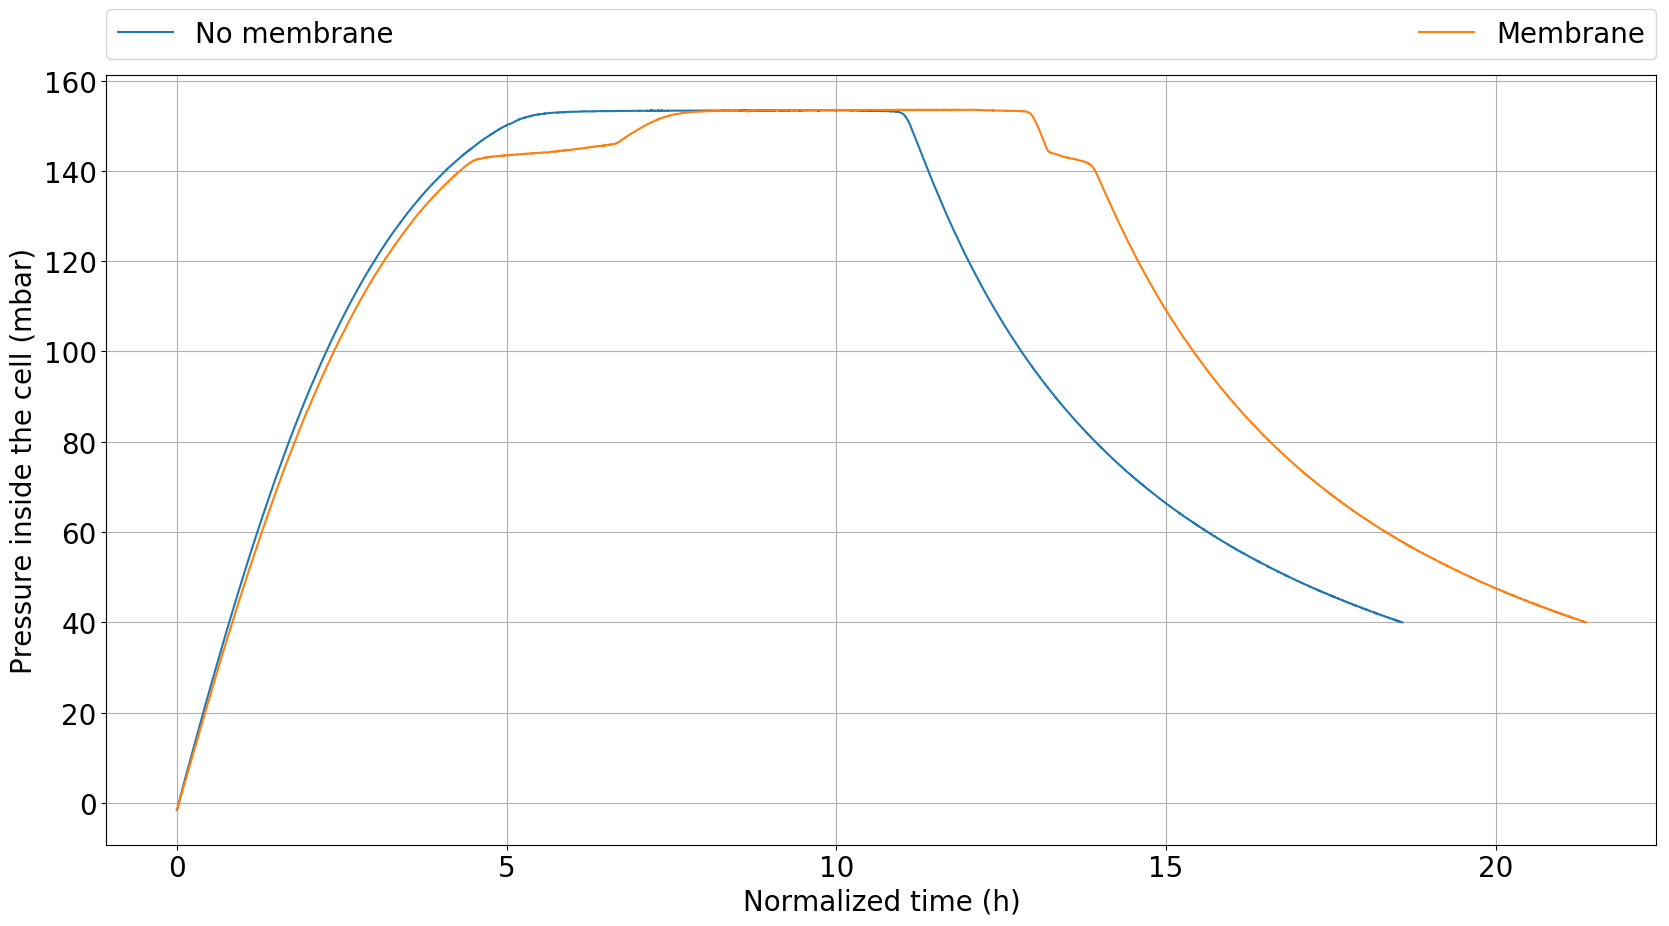
\includegraphics[width=\textwidth]{images/t.png}
            \label{fig:p-over-t}}\\
            \subfloat[]{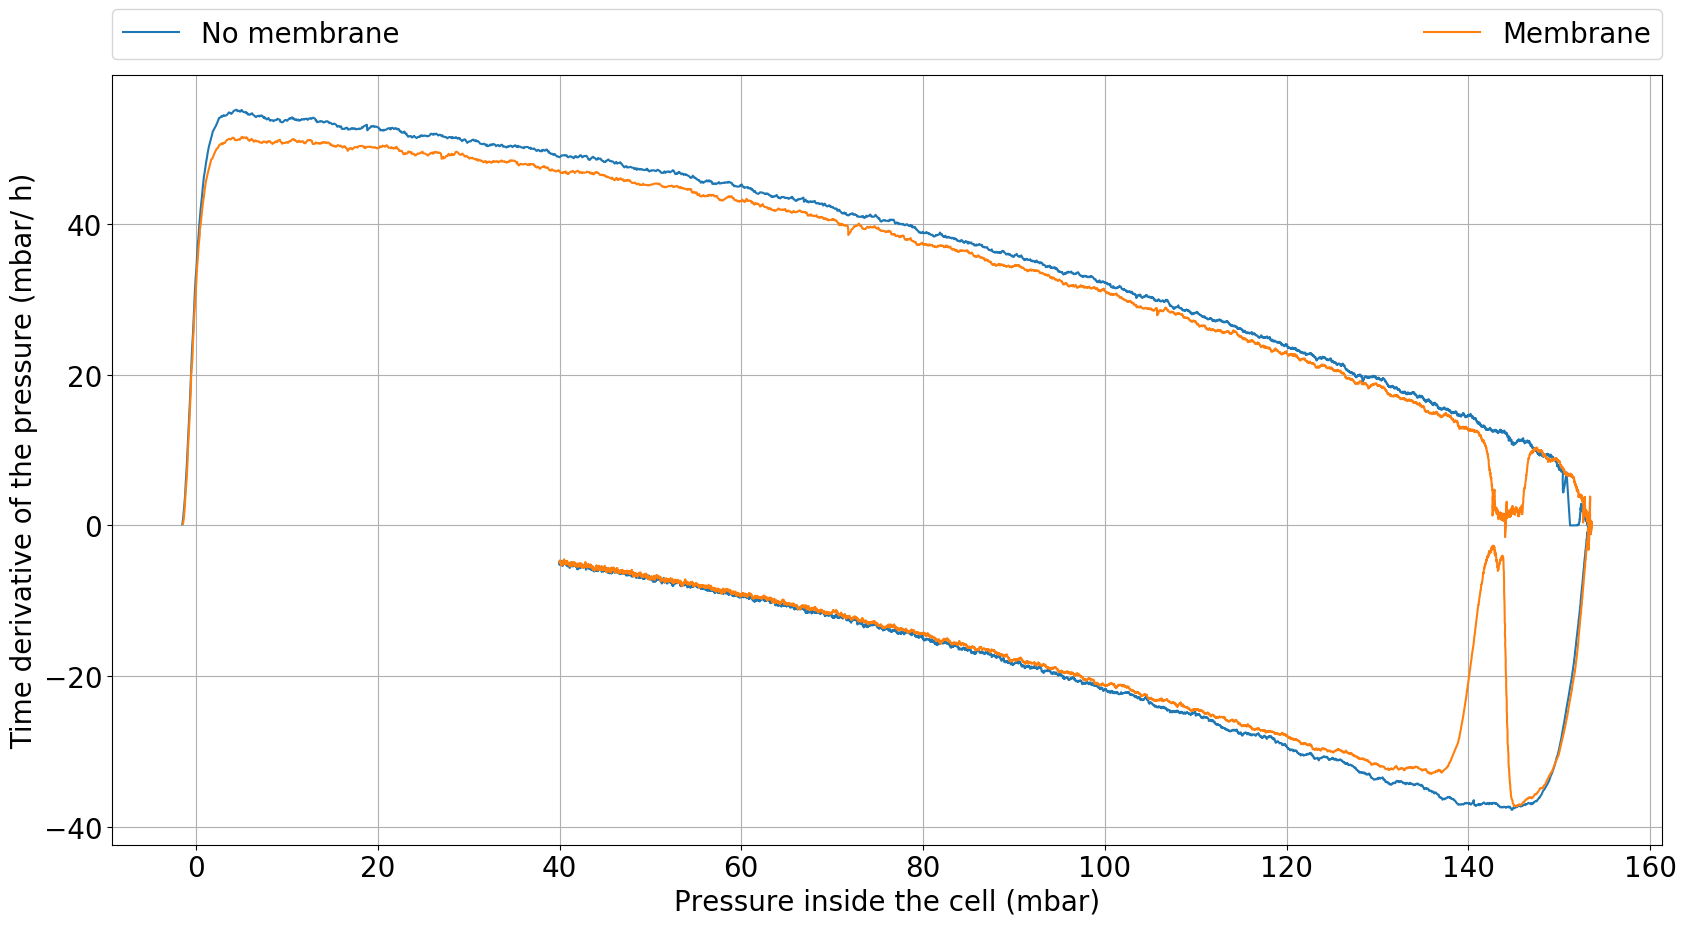
\includegraphics[width=\textwidth]{images/p.png}
            \label{fig:pressure-loop}}
            \caption{Raw volumetric isotherm data recorded with the experimental setup as explained in \cref{sec:experimental-procedure} for one cycle without a membrane inside the cell and one with a membrane inside the cell. \protect\subref{fig:p-over-t} shows the pressure values over time making the condensation and evaporation plateaus of absorption and desorption of hexane within the membrane's pores visible. \protect\subref{fig:pressure-loop} is the pressure loop which is relevant for the computation of the isotherms. Again, the before mentioned plateaus are visible as dips in the time derivative of the pressure. }
            \label{fig:raw-isotherms}
        \end{figure}

        Regarding the system with and empty cell, it is clear that the ideal gas law can be used to compute the flow rate of hexane (compare \cref{sec:ideal-gas-law}). By solving for the amount of matter
        \begin{equation*}
            n_1 = \frac{P_1V_1}{RT_1},
        \end{equation*}
        taking into account that the temperature of the cell is regulated at $T_1$ and the volume $V_1$ is constant, the flow of matter becomes
        \begin{equation*}
            \dot{n}_1 = \frac{V_1}{RT_1}\cdot \dot{P}_1.
            \label{eq:n1}
        \end{equation*}
        Furthermore, the flow of matter for the system with a membrane inside the cell can be interpreted as the sum of the flow into the membrane $\dot{n}_2^\mathrm{mem}$ and the flow into the system volume excluding the membrane $\dot{n}_2^\mathrm{cell}$. This can be rewritten yielding
        \begin{equation*}
            \dot{n}_2^\mathrm{mem} = \dot{n}_2 - \dot{n}_2^\mathrm{cell},
        \end{equation*}
        where $\dot{n}^\mathrm{cell}_2$ obeys ideal gas law. Using the fact that the flow through the \textsc{Pfeiffer} valve only depends on the pressure difference $\Delta P_i = P_i^\mathrm{tank} - P_i^\mathrm{cell}$, assuming that $P_1^\mathrm{tank} = P_2^\mathrm{tank}$ leads to
        \begin{align}
            \begin{split}
                \dot{n}_2^\mathrm{mem}(P_2) &= \dot{n}_1(P_2) - \dot{n}_2^\mathrm{cell}(P_2)\\
                &=\frac{V_1}{RT_1}\cdot \dot{P}_1(P_2) - \frac{V_2}{RT_2}\cdot \dot{P}_2(P_2)
            \end{split}
            \label{eq:ndot-membrane}
        \end{align}
        \Cref{fig:iso-computation} shows the computation steps visually using the respective plots versus time.

        \begin{figure}[ht]
            \centering
            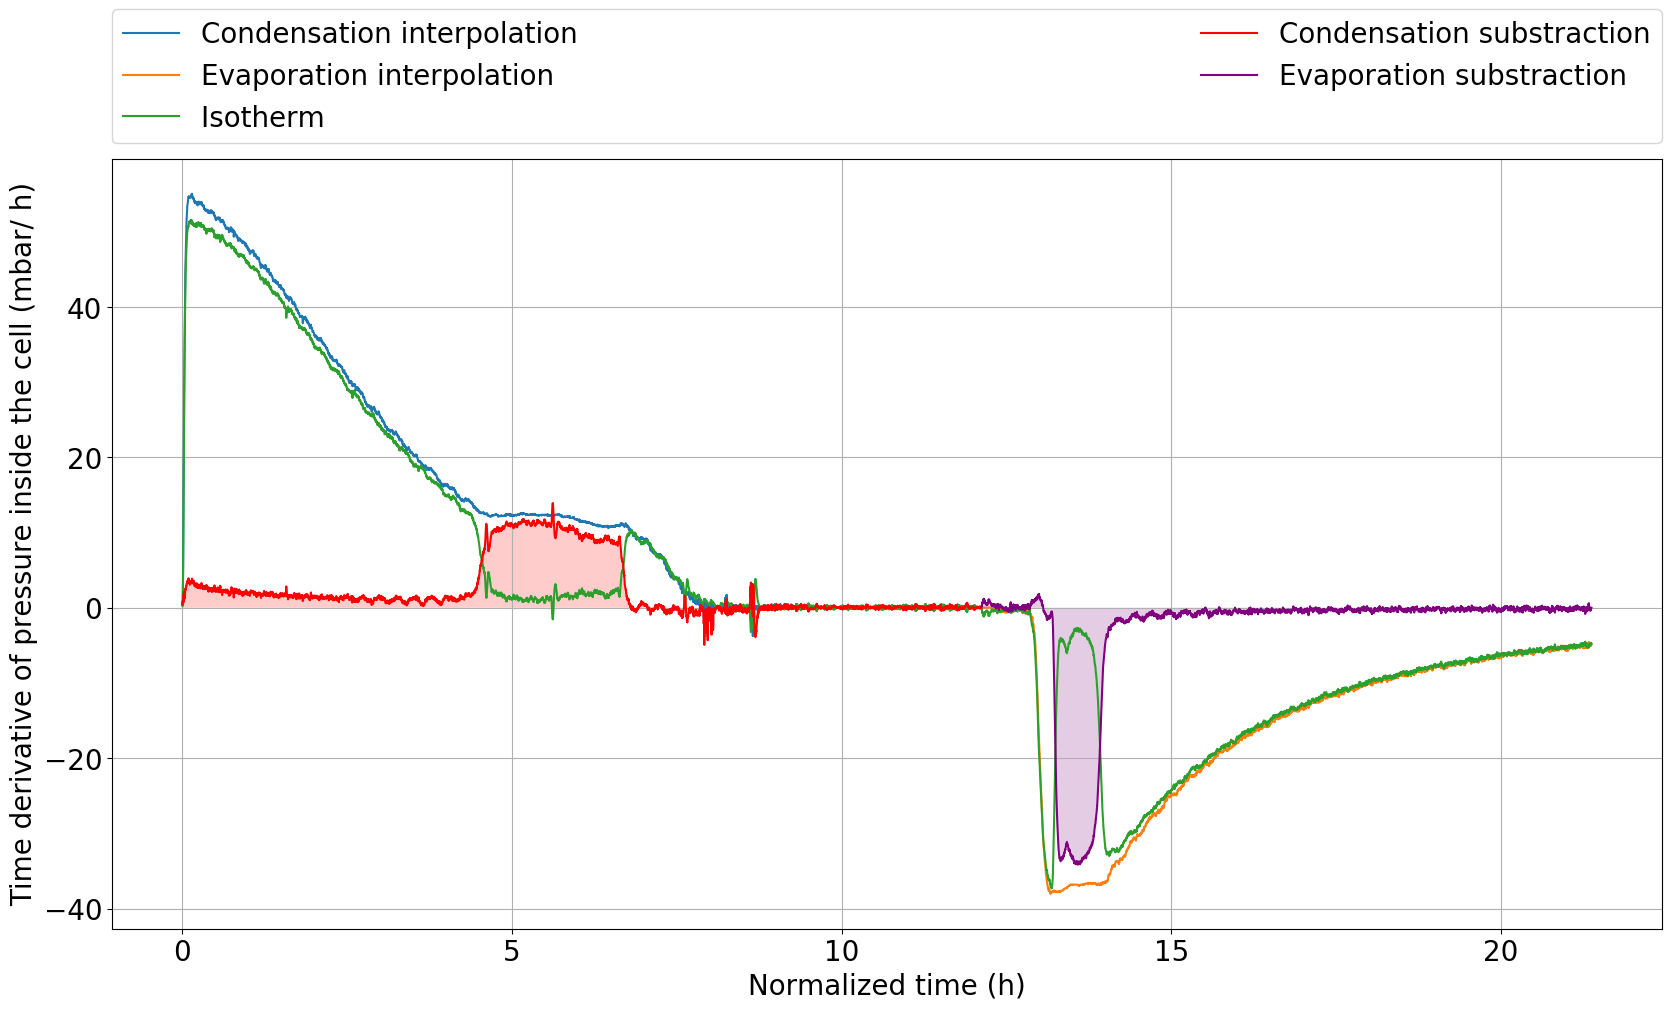
\includegraphics[width=\textwidth]{images/isotherm_comparison_report.png}
            \caption{Raw data of the isotherm with membrane and interpolation of the reference isotherm without membrane. Also, the substraction of the latter (compare integrand of \cref{eq:ndot-membrane}) is plotted where the area to be integrated for the absorption and respective desorption isotherm is shaded. }
            \label{fig:iso-computation}
        \end{figure}

        As the temperature of the system is regulated ($T = T_1 = T_2 = \mathrm{const.}$) and because $V = V_1 \approx V_2$ since $V_\mathrm{mem} \ll V_1$, equation \cref{eq:ndot-membrane} yields
        \begin{equation}
            n_2^\mathrm{membrane} = \frac{V}{RT}\int_0^{t_2}\left(\dot{P}_1(t_1') - \dot{P}_2(t_2')\right) \mathrm{d}t_2'.
            \label{eq:nmembrane}
        \end{equation}
        Important at this point is the dependency of $\dot{P}_1(t_1)$ on $t_1)$ while the integration is over $t_2$.

        As the experimental setup yields discreet values at given time intervals $\Delta t$, the data evaluation makes use of a sum rather than an integration.
        \begin{equation}
            n = \frac{V}{RT} \sum \left( \dot{P}_1 ( P_1 = P_2) - \dot{P}_2(P_2) \right) \cdot \Delta t
            \label{eq:nmembrane}
        \end{equation}
        yields the molar amount of hexane condensed inside the membrane. Figure \cref{fig:computed-isotherm} shows the result of the integration \cref{eq:nmembrane} for membrane 296d. It is a absorption and desorption isotherm for hexane inside the porous alumina membrane. The bulk condensation and evaporation is not visible, as it is also recorded with the reference isotherm without membrane inside the cell.
        \medskip

        Moreover, the plots
        \begin{equation}
            i \quad \mathrm{over} \quad j,\quad i\in \{n,LF,FF\}, \quad j\in \{P_\mathrm{cell},P_\mathrm{rel},D_\mathrm{kelvin}\}
        \end{equation}
        are of interest, where
        \begin{equation}
            P_\mathrm{rel} = \frac{P_\mathrm{cell}}{P_\mathrm{sv}^\mathrm{exp}},
        \end{equation}
        with the saturated vapor pressure $P_\mathrm{sv}$.
        \begin{equation}
            LF = \frac{n}{n_\mathrm{max}}
        \end{equation}
        is the liquid fraction of hexane condensed inside the pores of the membrane using the total maximum amount of condensed hexane $n_\mathrm{max}$ and last,
        \begin{equation}
            FF = \frac{V_\mathrm{hex}^\mathrm{cond}}{V_\mathrm{mem}}
        \end{equation}
        with the volume of condensed hexane $V_\mathrm{hex}^\mathrm{cond}$ and the membrane's volume $V_\mathrm{mem}$, is the filled fraction of the membrane. Its maximum corresponds to the porosity of the membrane. For the computation please refer to \cref{subsec:porosity}.

        For the computation of the introduced physical sizes, the saturated vapor pressure $P_\mathrm{sv}$ must be determined.

        \begin{figure}[ht]
            \centering
            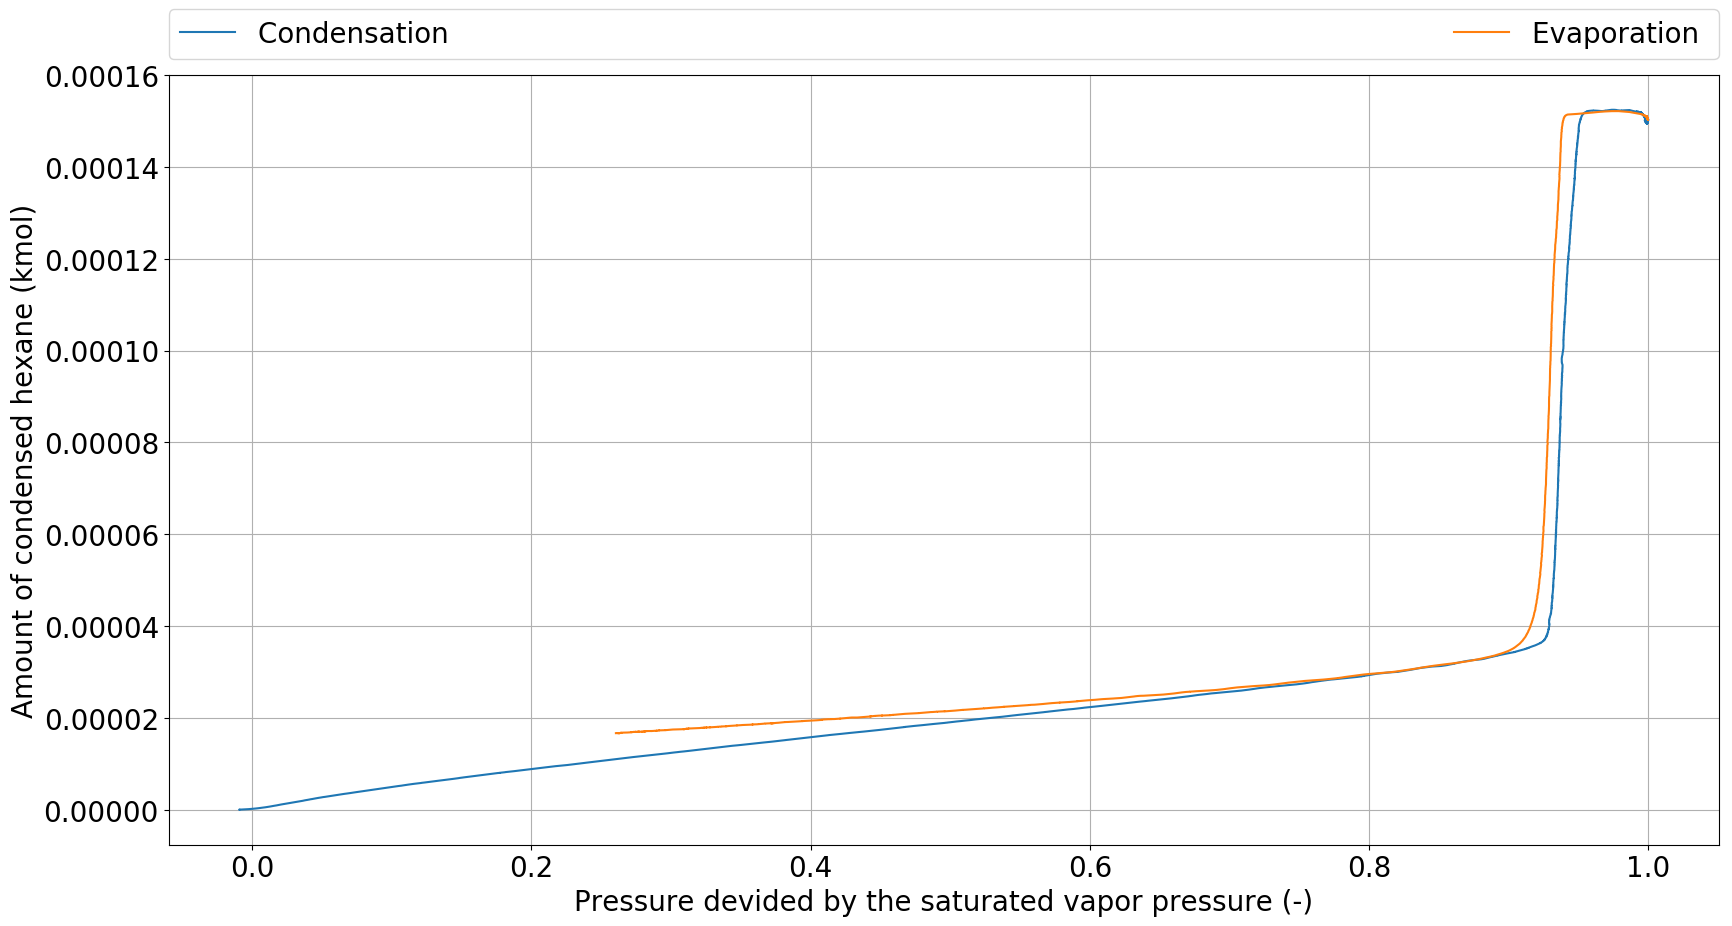
\includegraphics[width=\textwidth]{images/prel_isotherm_computation.png}
            \caption{Isotherm computed using equation \cref{eq:nmembrane}. The pressure axis has been divided by the saturated vapor pressure. }
            \label{fig:computed-isotherm}
        \end{figure}


        \subsection{Determination of the Saturated Vapor Pressure}

            As the bulk condensation plateau shows a slight drift (compare figure \cref{fig:raw-isotherms}), using the maximum measured pressure $P_\mathrm{cell}$ does not yield the saturated vapor pressure $P_\mathrm{sv}$ but a higher value. In addition, depending on the contamination of the system by air or degassing grease, the measured value for $P_\mathrm{sv}$ shifts due to the partial pressures. To probe the reproducibility of an isotherm loop including the grade of contamination, the maximum measured pressure for different membranes is compared. As the system is opened to replace the membrane in between the isotherms, each cycle is independent. For the change of membrane process please read \cref{sssec:changing-the-sample}. The result of the experiment is that $P_\mathrm{sv}^\mathrm{exp}$ fluctuates by
            \begin{equation}
                \delta P_\mathrm{sv}^\mathrm{exp} = \pm \SI{0,5}{\milli\bar}.
                \label{eq:delta-Psat}
            \end{equation}
            As the relevant plateau of condensation and evaporation inside the pores of the membrane occur at about
            \begin{equation}
                P_\mathrm{plateaus} = \SI{140}{\milli\bar},
            \end{equation}
            $\delta P_\mathrm{sv}^\mathrm{exp}$ translates to an error of about
            \begin{equation}
                \delta P_\mathrm{rel} \le \pm 0,005.
                \label{eq:delta-Prel}
            \end{equation}


        \subsection{Porosity}
        \label{subsec:porosity}

            Equation \cref{eq:nmembrane} gives the molar amount of hexane $n_\mathrm{hex}$ condensed inside the membrane's pores. Furthermore, for the given pressures $\SIrange{0}{160}{\milli\bar}$ hexane in its liquid form can be regarded as incompressible and therefore the hexane's volume be computed via
            \begin{equation*}
                V_\mathrm{hex} = n_\mathrm{hex} \cdot V_\mathrm{mol, hex}.
            \end{equation*}.
            The thickness $l_\mathrm{pore}$ of the membrane is easily determinable via MEB views since its magnitude is micrometers. Finally, the area $A_\mathrm{mem}$ of the measured samples is derived from a photo taken using binoculars.

            Using these information the porosity $\phi$ of a given membrane is given by
            \begin{equation}
                \phi = 1 - \frac{V_\mathrm{hex}}{V_\mathrm{mem}} ,
                \label{eq:porosity}
            \end{equation}
            with the membrane's volume
            \begin{equation*}
                V_\mathrm{mem} = A_\mathrm{mem} \cdot l_\mathrm{pore}.
            \end{equation*}


        \subsection{Light Transmission Evaluation}
        \label{subsec:light-transmission-evaluation}

            As mentioned in \cref{sec:exp-setup}, the light transmission setup is independent from the volumetric measurements and also the evaluations do not depend on each other. The light transmission is rather a tool to check on the theory of evaporation and condensation within the membrane using a different approach.
            \medskip

            To compute the transmission coefficient of a membrane, it is measured in dry state using the same transmission setup as during the volumetric experiment yielding $T_\mathrm{mem}^\mathrm{dry}$. Then, the first measured intensity value $I_0$ of a given isotherm is assigned to the dry coefficient as at this point no hexane is condensed inside of the membranes pores yet. From there on, each intensity measurement is translated to a transmission coefficient according to
            \begin{equation}
                T(t) = T_\mathrm{mem}^\mathrm{dry} \cdot \frac{I_0}{I(t)}.
            \end{equation}
            The aquired physical size can be interpreted as explained in the following  \cref{subsec:light-transmission-interpretation}.


            \subsubsection{Light Transmission Interpretations}
            \label{subsec:light-transmission-interpretation}

                \subfile{tikz/transmission_disorder/pore_disorder.tex}

                Firstly, a completely filled membrane should always yield a higher transmission coefficient $T$ than in its dry state according to the theory of index matching explained in \cref{sec:index-matching}. This fact serves as a tool to optically detect membranes that do not fill completely due to constrictions.

                Furthermore, due to the disorder created by pore filling and emptying, the transmission drops during the processes. Phenomena occurring on the volumetric measurements can therefore be interpreted corresponding to the measured transmission coefficient.

                Last, an often observed phenomenon is that the transmission drops to lower values for the condensation than for evaporation of a given isotherm. \Cref{fig:transmission-drops} shows an isotherm of membrane 292d (open pores) where this is the case. A possible interpretation is the degree of disorder caused inside the membrane by the respective process. As the membrane contains pores open on both ends, the condensation takes place at spinodal pressure $P_\mathrm{sp}(d_\mathrm{pore})$. Due to the distribution of pore sizes, funnelization, corrugation and constrictions, the pores fill at different pressures $P_\mathrm{sp}^1 \neq P_\mathrm{sp}^2$. At a given pressure
                \begin{equation*}
                    P_\mathrm{sp}^1 < P < P_\mathrm{sp}^2,
                \end{equation*}
                where $P_\mathrm{sp}^1$ shall be the smallest pore diameter to be found on the membrane and $P_\mathrm{sp}^2$ the largest one, the state of the me{}mbrane regarding filled and empty pores is assumed to be comparable to figure \cref{fig:pore-disorder} \protect\subref{fig:disorder-absorption}.

                The hexane evaporates at equilibrium pressure $P_\mathrm{eq}$, though. That means that assuming the same pore size distribution, funnelization, corregation and constrictions, the pores empty continuously. The theoretical state of the membrane is visualized in \cref{fig:pore-disorder} \protect\subref{fig:disorder-desorption}.
                \medskip

                \begin{figure}[ht]
                    \centering
                    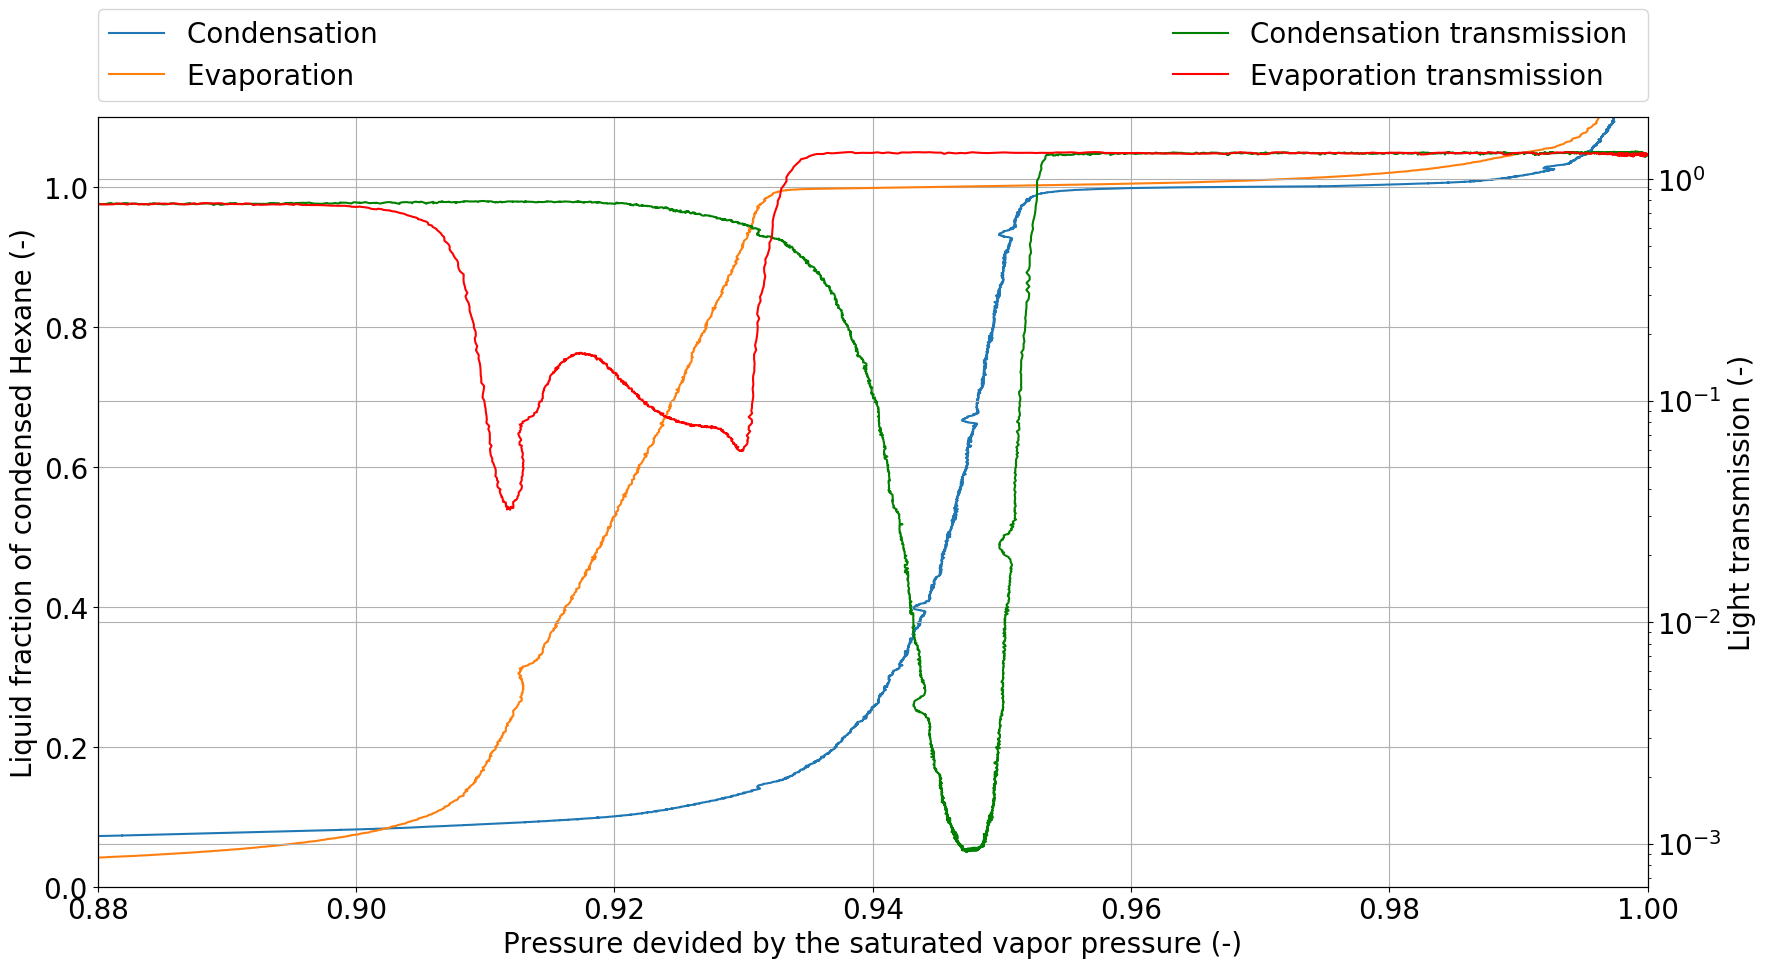
\includegraphics[width=\textwidth]{images/transmission_magnitude.png}
                    \caption{$P_\mathrm{rel}$ isotherm of membrane 292d. The transmission is not normalized but in arbitrary units plotted on a log scale. Please refer to \cref{subsec:light-transmission-interpretation} for the interpretation of the different magnitudes of the transmission drops for absorption and desorption. }
                    \label{fig:transmission-drops}
                \end{figure}

                The difference is that during the condensation process neighboring pores can be in very different states meaning empty and filled, while for evaporation the pores only show different levels of liquid during most of the process. Therefore, the absorption of hexane creates a higher grade of disorder than the desorption and therefore causes a more significant drop of the transmission coefficient (compare \cref{fig:transmission-drops}).
                \medskip

                The occurrence of the small peak in between two dips of the evaporation transmission cannot be explained by this theory. Moreover, the later analysed membranes of wafer 295 yield a more even dip distribution and upon reducing the pore diameter using ALD, even the membranes even show the inverse behaviour. ??? ADD THE FIGURE HERE



\end{document}
